%\documentclass[12pt]{scrbook}
%
%\usepackage{tikz}
%\usepackage{minted}
%\usetikzlibrary{decorations.pathreplacing,arrows}
%\usetikzlibrary{arrows,decorations.pathmorphing,backgrounds,positioning,fit,petri}
%
%\usepackage{fullpage}
%\usepackage{subfigure}
%\begin{document}
%
%
%Lorem Ipsum is simply dummy text of the printing and typesetting industry. Lorem Ipsum has been the industry's standard dummy text ever since the 1500s, when an unknown printer took a galley of type and scrambled it to make a type specimen book. It has survived not only five centuries, but also the leap into electronic typesetting, remaining essentially unchanged. It was popularised in the 1960s with the release of Letraset sheets containing Lorem Ipsum passages, and more recently with desktop publishing software like Aldus PageMaker including versions of Lorem Ipsum.





\begin{figure}
\centering

\subfigure[First iteration.  42 is chosen as the pivot element.  The index
variable $i$ moves over to 102, the first element that is greater than 42 and
on the ``wrong'' side of the partition.  The $j$ index variable does not
move as 0 is less than the pivot element and on the wrong side; these
are swapped.]{

\begin{tikzpicture}[scale=.65,transform shape]

%\tikzset{>=stealth',shorten <=.2cm,>=stealth',shorten >=.2cm}
% size of each node
\def\sz{9mm}
% node style definition
\tikzstyle{block} = [
	draw, fill=black!10, rectangle,
	minimum height=\sz, minimum width=\sz ];
\tikzstyle{plain} = [draw=none,fill=none];

%\node[plain] at (-1.75, 1) { index };
%\node[plain] at (0*\sz,1.0) { 0 };
%\node[plain] at (1*\sz,1.0) { 1 };
%\node[plain] at (2*\sz,1.0) { 2 };
%\node[plain] at (3*\sz,1.0) { 3 };
%\node[plain] at (4*\sz,1.0) { 4 };
%\node[plain] at (5*\sz,1.0) { 5 };
%\node[plain] at (6*\sz,1.0) { 6 };
%\node[plain] at (7*\sz,1.0) { 7 };
%\node[plain] at (8*\sz,1.0) { 8 };
%\node[plain] at (-1.75, 0) { contents };
%

\node[block,fill=green!50] (a0) at (0*\sz,0) { 42 };
\node[block] (a1) at (1*\sz,0) { 4 };
\node[block] (a2) at (2*\sz,0) { 9 };
\node[block] (a3) at (3*\sz,0) { 4 };
\node[block] (a4) at (4*\sz,0) { 102 };
\node[block] (a5) at (5*\sz,0) { 34 };
\node[block] (a6) at (6*\sz,0) { 12 };
\node[block] (a7) at (7*\sz,0) { 2 };
\node[block] (a8) at (8*\sz,0) { 0 };

\node[below of=a1] (c1) {};
\node[below of=a2] (c2) {};
\node[below of=a3] (c3) {};
\node[below of=a4] (c4) {};
\draw[->] (c1) -- (a1);
\draw[->] (c2) -- (a2);
\draw[->] (c3) -- (a3);
\draw[->] (c4) -- (a4);

\draw[->,dotted] (c1) -- (c2);
\draw[->,dotted] (c2) -- (c3);
\draw[->,dotted] (c3) -- (c4);

\node[below of=a8] (d1) {};
\draw[->] (d1) -- (a8);
\node[below of=d1,above] {$j$};

\draw [decorate,decoration={brace,mirror,amplitude=5pt},xshift=-4pt,yshift=0pt] ([xshift=0cm,yshift=0cm]c1.south) -- ([xshift=0cm,yshift=0cm]c4.south) node [black,midway,yshift=-0.75cm] {$i$};

\draw[<->,>=stealth',shorten <=.2cm,>=stealth',shorten >=.2cm] (a4.south) to [bend right] node[pos=.5,below] {swap} (a8.south);

%\draw[<->] (a4.south) to [in=270,out=270,looseness=1] node[pos=.5,below] {swap} (a8.south);

\end{tikzpicture}~~~~~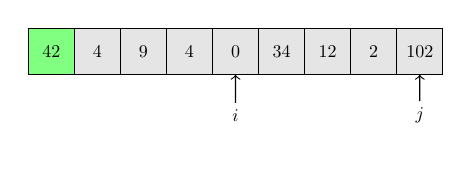
\begin{tikzpicture}[scale=.65,transform shape]

\def\sz{9mm}
\tikzstyle{block} = [
	draw, fill=black!10, rectangle,
	minimum height=\sz, minimum width=\sz ];
\tikzstyle{plain} = [draw=none,fill=none];
\draw[white] (0,0) rectangle (1, -2.15);

\node[block,fill=green!50] (a0) at (0*\sz,0) { 42 };
\node[block] (a1) at (1*\sz,0) { 4 };
\node[block] (a2) at (2*\sz,0) { 9 };
\node[block] (a3) at (3*\sz,0) { 4 };
\node[block] (a4) at (4*\sz,0) { 0 };
\node[block] (a5) at (5*\sz,0) { 34 };
\node[block] (a6) at (6*\sz,0) { 12 };
\node[block] (a7) at (7*\sz,0) { 2 };
\node[block] (a8) at (8*\sz,0) { 102 };

\node[below of=a4,node distance=1.25cm] (c4) {$i$};
\draw[->] (c4) -- (a4);
\node[below of=a8,node distance=1.25cm] (d1) {$j$};
\draw[->] (d1) -- (a8);

\end{tikzpicture}

}

\subfigure[Second iteration.  The index variable $i$ moves all the way to the
right as all remaining elements are less than the pivot, 42.  The index
variable $j$ remains at 102 as $i$ is now equal to $j$.  The pivot, 
42 is placed between the two partitions and its resulting index, $s$
is returned.]{

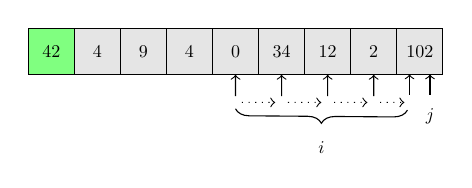
\begin{tikzpicture}[scale=.65,transform shape]

%\tikzset{>=stealth',shorten <=.2cm,>=stealth',shorten >=.2cm}
% size of each node
\def\sz{9mm}
% node style definition
\tikzstyle{block} = [
	draw, fill=black!10, rectangle,
	minimum height=\sz, minimum width=\sz ];
\tikzstyle{plain} = [draw=none,fill=none];

%\node[plain] at (-1.75, 1) { index };
%\node[plain] at (0*\sz,1.0) { 0 };
%\node[plain] at (1*\sz,1.0) { 1 };
%\node[plain] at (2*\sz,1.0) { 2 };
%\node[plain] at (3*\sz,1.0) { 3 };
%\node[plain] at (4*\sz,1.0) { 4 };
%\node[plain] at (5*\sz,1.0) { 5 };
%\node[plain] at (6*\sz,1.0) { 6 };
%\node[plain] at (7*\sz,1.0) { 7 };
%\node[plain] at (8*\sz,1.0) { 8 };
%\node[plain] at (-1.75, 0) { contents };
%

\node[block,fill=green!50] (a0) at (0*\sz,0) { 42 };
\node[block] (a1) at (1*\sz,0) { 4 };
\node[block] (a2) at (2*\sz,0) { 9 };
\node[block] (a3) at (3*\sz,0) { 4 };
\node[block] (a4) at (4*\sz,0) { 0 };
\node[block] (a5) at (5*\sz,0) { 34 };
\node[block] (a6) at (6*\sz,0) { 12 };
\node[block] (a7) at (7*\sz,0) { 2 };
\node[block] (a8) at (8*\sz,0) { 102 };

\node[below of=a4] (c4) {};
\node[below of=a5] (c5) {};
\node[below of=a6] (c6) {};
\node[below of=a7] (c7) {};
%\node[below of=a8,xshift=-10pt] (c8) {};
\draw[->] (c4) -- (a4);
\draw[->] (c5) -- (a5);
\draw[->] (c6) -- (a6);
\draw[->] (c7) -- (a7);

\draw[->,dotted] (c4) -- (c5);
\draw[->,dotted] (c5) -- (c6);
\draw[->,dotted] (c6) -- (c7);
\draw[->,dotted] (c7) -- (6.9,-1.0);

\node[below of=a8] (d1) {~};
\draw[->] (7.4,-0.85) -- (7.4,-0.45);
\draw[->] (7.0,-0.85) -- (7.0,-0.45);
\node[below] at (7.4, -1) {$j$};

\draw [decorate,decoration={brace,mirror,amplitude=5pt},xshift=-4pt,yshift=0pt] ([xshift=0cm,yshift=0cm]c4.south) -- (7.1,-1.15) node [black,midway,yshift=-0.75cm] {$i$};

%\draw[<->,>=stealth',shorten <=.2cm,>=stealth',shorten >=.2cm] (a4.south) to [bend right] node[pos=.5,below] {swap} (a8.south);

%\draw[<->] (a4.south) to [in=270,out=270,looseness=1] node[pos=.5,below] {swap} (a8.south);

\end{tikzpicture}~~~~~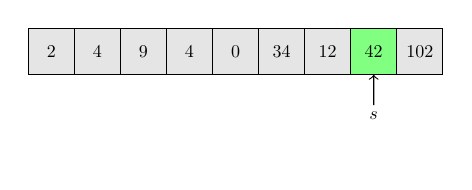
\begin{tikzpicture}[scale=.65,transform shape]

\def\sz{9mm}
\tikzstyle{block} = [
	draw, fill=black!10, rectangle,
	minimum height=\sz, minimum width=\sz ];
\tikzstyle{plain} = [draw=none,fill=none];
\draw[white] (0,0) rectangle (1, -2.15);

\node[block] (a0) at (0*\sz,0) { 2 };
\node[block] (a1) at (1*\sz,0) { 4 };
\node[block] (a2) at (2*\sz,0) { 9 };
\node[block] (a3) at (3*\sz,0) { 4 };
\node[block] (a4) at (4*\sz,0) { 0 };
\node[block] (a5) at (5*\sz,0) { 34 };
\node[block] (a6) at (6*\sz,0) { 12 };
\node[block,fill=green!50] (a7) at (7*\sz,0) { 42 };
\node[block] (a8) at (8*\sz,0) { 102 };

%\node[below of=a4,node distance=1.25cm] (c4) {$i$};
%\draw[->] (c4) -- (a4);
\node[below of=a7,node distance=1.25cm] (d1) {$s$};
\draw[->] (d1) -- (a7);

\end{tikzpicture}

}

\caption[Partitioning Example 1]{Example execution of the \textsc{Partition}
subroutine in Quick Sort.  A total of 8 comparisons are made, 9 if you count
the last swap outside the while loop.  The partition returns $s$ as the
pivot position; the right-partition is sorted as it only consists of 1 element.}
\label{figure:partitionExample1}

\end{figure}


%\end{document}

